\documentclass[11pt]{article}

% PACKAGE USING
\usepackage[top = 1in, bottom = 1in, left = 0.75in, right = 0.75in]{geometry}
\usepackage{amsmath, amssymb, amsthm, amsfonts}
\usepackage{xcolor}
\usepackage{graphicx, subcaption}
\usepackage{url, hyperref}
\hypersetup{
    colorlinks = true,
    urlcolor = blue,
    citecolor = red
}
%\usepackage{biblatex}
%\addbibresource{references.bib}


\newcommand{\Q}{\mathbb{Q}}
\newcommand{\E}{\mathbb{E}}
\newcommand{\R}{\mathbb{R}}
\newcommand{\Acal}{\mathcal{A}}
\newcommand{\Fcal}{\mathcal{F}}
\newcommand{\transpose}{^{\intercal}}
\newcommand{\prob}{\mathbb{P}}
\newcommand{\ind}[1]{\boldsymbol{1}\{#1\}}

\newtheorem{example}{Example}



\begin{document}

\begin{titlepage}
    \begin{center}
        \vspace*{5cm}
 
        \Huge{\textbf{Extension of Research Reading Assignment}}
 
        \vspace{0.5cm}
        \large{of the paper titled}\\
        \large{``Correlated Bandits for Dynamic Pricing via the ARC algorithm''}\\
        \large{by}\\
        \large{Samuel N. Cohen and Tanut Treetanthiploet}
             
        \vspace{1.5cm}
 
        \large{\textit{Prepared by,}}\\
        \large{\textbf{Subhrajyoty Roy}}\\
        \large{\textbf{MB1911}}
 
        \vspace{2cm}
             
        \textit{Assignment for Computational Finance course\\
        as a part of Master of Statistics curriculum}\\
        \vspace{0.5cm}
        \textbf{Session: } 2020-21\\
        Indian Statistical Institute, Kolkata

        \vfill
        
        \begin{flushright}
            \normalsize{\today}            
        \end{flushright}
    \end{center}
\end{titlepage}


\section{Introduction}

The multi-armed bandit problem (or the classical $K$-armed bandit problem)~\cite{katehakis1987multi} is a problem derived from reinforcement learning theory, which shows the most typical example of ``exploitation'' and ``exploration'' trade-off dilemma. In its original version, the problem starts with a gambler at a casino with a finite amount of money. The casino has $k$ slot machines, each giving a random reward at each time based on different probabilities of winning. The gambler is faced off with the problem of allocating his (or her) resources in a way to maximize his (her) ultimate gain. Typical two extreme scenarios would be 

\begin{enumerate}
    \item The gambler plays only one slot machine to ``exploit'' its weakness, which could lead to potential loss of winning higher rewards from other slots machines he (she) never played.
    \item The gambler plays randomly all of the machines to ``explore'' their probability of winnings. But he (she) ends up using too many resources to estimate, hence losing any strategy to gain more than the expected value.
\end{enumerate}

Although the problem is only theoretically posed as a probability question, it has enormous real-life applications. A survey on these practical applications is available by Bouneffouf and Rish~\cite{bouneffouf2019survey}, some of them are mentioned below.

\begin{example}\label{example:1}
    An agent commutes from home to work every morning. She would like to commute along the path that requires the least average travel time, but she is uncertain of the travel time along different routes. How can she learn efficiently and minimize the total travel time over a large number of trips?

    \begin{figure}[ht]
        \centering
        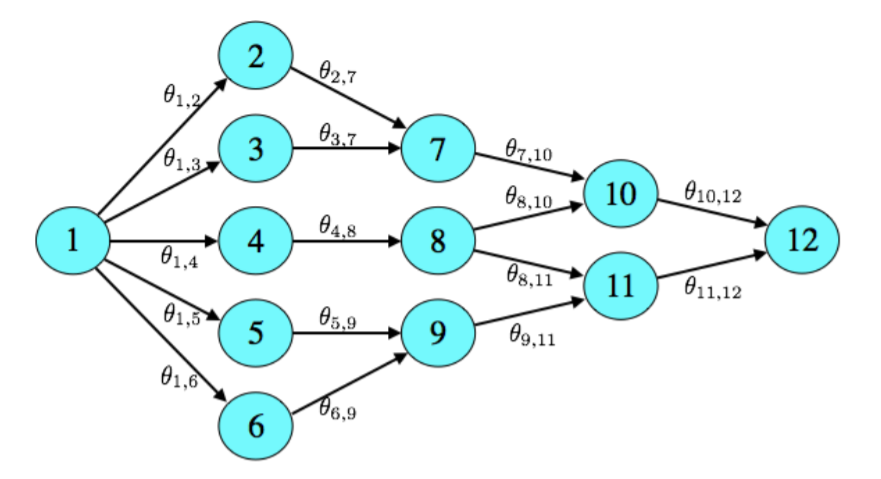
\includegraphics[width = 0.8\textwidth]{travel-example.png}
    \end{figure}

    We formulate this problem with a graph $G = (V, E)$, where each edge has an associated parameter $\theta_{e}$. At day $t$, when she takes edge $e$ as the route, then it takes $y_{t, e} \sim F(\theta_e)$ time through that edge. However, she only observes $\sum_{e \in \text{her path}} y_{t, e}$ for each day, which is the negative reward. This is again a multi-armed bandit problem where the reward itself may be a function of multiple parameters.
\end{example}

\begin{example}\label{example:2}
    An investor needs to find the optimal portfolio to invest in the stock market. There are many available portfolios $H_1, H_2, \dots H_k$, each of which pays a different reward which is stochastic and dynamic in nature, i.e. $H_i$ pays a reward of $R_{i,t}$ at time $t$ governed by some underlying parameter $\theta_{i}$. However, sticking with a single optimal portfolio for a longer period would make every investor in the market aware of its existence, and hence the demand for that particular portfolio would continue to rise. Because of the usual demand-supply equation, the price of the portfolio would continue to rise and the optimal portfolio would not remain profitable enough. Therefore, the investor needs to allocate his (her) resources with utmost care to ensure long term profitability.
\end{example}

\begin{example}\label{example:3}
    Online retailer companies are often faced with the dynamic pricing problem: the company must decide on real-time prices for each of its multiple products. Let, $p_1, p_2, \dots p_k$ be the $k$ choice of prices of the items, with the demand function being $\theta(p_i) \in (0, 1)$. However, if only $N_t$ people visits that store on day $t$ which is random, only $Y_{t, i} \sim \text{Bin}(N_t, \theta(p_i))$ is the number of people to buy that product at price $p_i$ on day $t$. Therefore, the reward or the revenue turns out to be $p_i Y_{t, i}$, which we want to maximize. In contrast to the example before, here, knowledge of the reward is the same as the knowledge of the random response $Y_{t, i}$ from the system. 
\end{example}


\section{Existing Approaches}

There are numerous approaches to solve the multi-armed bandit problem as follows.

The most naive algorithm is the Greedy algorithm which always takes the action that maximizes the reward. Therefore, if there are $K$ slot machines, the first $K$ trials are used to explore their ``rewards" distribution. From then onwards, the most profitable action is chosen in each round and based on the rewards obtained, the inference about each of the slot machine is continuously updated. However, as it has been shown, this procedure may get stuck to a suboptimal solution~\cite{russo2017tutorial}.

A better version if $\epsilon$-greey algorithm~\cite{vermorel2005multi} in which the gambler may take the greedy action with probability $(1 - \epsilon)$, but with the rest of the probability $\epsilon$, he (she) chooses any other action uniformly picked at random. This ensures a balance between exploring rewards from new actions to ensure that the inference about the unknown parameters is always updated. However, this procedure wastes a large number of resources hence could take a longer time to reach optimality. 

Another variant of the greedy algorithm is Explore-then-commit algorithm~\cite{rusmevichientong2010linearly}. According to this strategy, explores randomly for $[\epsilon T]$ rounds which are only used to update inference about the reward distributions, and then it keeps taking the greedy action only. In this case, the choice of $\epsilon$ is crucial in ensuring the optimality of this approach.

Thompson sampling~\cite{thompson1933likelihood} calculates the posterior probability conditional on $\Fcal_{t-1}$ (i.e. the $\sigma$-field containing the history upto time $(t-1)$), that the action $a$ gives the maximum reward at time $t$. Then, it samples an action $a$ according to this probability distribution. In contrast to the Greedy algorithm, which maximizes the expected reward, Thompson sampling reverses the maximization and expectation step in the greedy algorithm.

Asymptotic Randomized Control~\cite{cohen2020asymptotic,treetanthiploet2021correlated} is another algorithm that works on the idea that the reward distributions of the slot machines are not necessarily independent, hence obtaining reward from one machine may reveal interesting characteristics of the other machines. For example, if there is a machine that gives lower rewards compared to other machines, but perfectly reveals the underlying common parameter (i.e. perfectly reveals the reward distributions of all the machines), then Thompson sampling will never choose this action. ARC (Asymptotic Randomized Control) strategy would consider the following discounted objective function to maximize 

$$V = \sum_{t=1}^\infty \beta^{(t-1)}\E_{a_t}(R(t, a_t)\mid \Fcal_{t-1})$$

\noindent where $\beta \in (0, 1)$ is a discounting rate, $a_t$ is the optimal action taken at time $t$, $R(t, a_t)$ is the reward at time $t$ for applying action $a_t$. Assuming that $\{ a_t \}$ is an optimal action to choose for the first round since infinitely many rounds are taken under consideration, the best action $\{ a_t \}$ still works as an optimal action for the remaining scenario as well, since the situation is the same as before except that the rewards are discounted by $\beta$ and the underlying parameter $\Theta \sim F(\theta)$ now follows the posterior distribution of $\Theta \sim F(\theta \mid \Fcal_1)$. Based on this idea, Cohen and Treetanthiploet~\cite{treetanthiploet2021correlated} showed that the optimal action can be obtained by solving the fixed point equation

$$
a_t = \E_{a_t}(R(t, a_t)\mid \Fcal_{t-1}) + \dfrac{\beta}{(1 - \beta)} L^\lambda(t, a_t)
$$

\noindent where $L^\lambda(t, a_t)$ is an ``exploration'' term which uses the derivatives of $\E_{a_t}(R(t, a_t)\mid \Fcal_{t-1})$, which under assumption of asymptotic normality (in generalized linear model setup) can be shown to be related to the precision of the posterior distribution. In this way, they suggest that this algorithm takes account of the amount of information gained into consideration.

\section{Objectives of the study}

The objective of this study is to explore two limitations of the usual assumptions made by Cohen~\cite{cohen2020asymptotic,treetanthiploet2021correlated} during the derivation of ARC algorithm.

\begin{enumerate}
    \item In Example~\ref{example:2} and~\ref{example:3}, the situation differs from the classical $k$-arm bandit problem in the way that after each round, the internal state of the slot machines changes. For instance, if a company finds a particular ad banner is making a much greater profit than other banners, they will continue to display it by the usual Thompson and ARC algorithms since it is optimal. However, the preferences of the population are not static, hence displaying the same ad banner over and over again would become hackneyed and encourage repulsive behaviour of the general populace.
    \item The discounted expected reward expects the number of rounds as countably infinite. However, in practicality, only a finite $T$ number of rounds are played, and the firm set a $T$ which will not be very large enough. This suggests that the fixed point equation in ARC algorithm will only be an approximation.
\end{enumerate}

\section{Mathematical Formulation and New Algorithm}

We would consider a very general setup which encompasses both Example~\ref{example:2} and \ref{example:3}. Let, $X_t$ be a latent parameter at time $t$ denoted by a $p$-dimenaional random vector. This latent vector $X_t$ could represent the preferences of the general public towards certain products, or could denote market conditions of the economy of the country. Let, this $X_t$ evolves according to a stochastic rule $X_{t+1} \sim f(X_t, a_t, \theta)$, where $a_t$ is the action chosen at time $t$. Clearly, the action $a_t$ chosen from the action space $\mathcal{A}$ has some effect in the latent conditions (or the environment on which the agent is acting upon), which makes the process similar to a feedback loop. Also, once action $a_t$ has been chosen, a random variable $Y_t \sim g(X_t, a_t, \eta)$ is observed and a deterministic function $R_t(Y_t)$ is the obtained reward. Let, $(\Omega, \prob, \Fcal)$ be the probability space on which these random variables are defined, and let $\Fcal_{t}$ be the natural filtration denoting the history upto time $t$.

Our goal would be to maximize the expected discounted reward $V$ with respect to the choice of actions $\{a_t\}_{t = 1}^{T}$,

$$
V(a_1, \dots a_T) = \sum_{t = 1}^T \beta^{(t-1)} \E(R_t(Y_t(a_t))), \qquad \text{ where } \beta \in (0, 1)
$$

The precise departure due to this finite time horizon is that, now the balance between exploration and exploitation need not be same for each round. For instance, in ARC algorithm, a parameter $\lambda$ was used to encourage exploration to find better actions, however, the choice of $\lambda$ is taken to be static throughout. However, due to finite time, first few rounds should encourage more exploration rather than exploitation, while the last few rounds should encourage exploitation. In particular, for the last $T$-th round, any reasonable agent (gambler) would never try to explore any further to search for more profitable actions, because that action, even if discovered, cannot be taken. Therefore, in the very last round, any reasonable agent (gambler) would only take the best possible action conditioned on the inference gained from the history of $(T-1)$ rounds. In formal terms, 

$$
a_T = \arg\max_{a \in \Acal} \E(R_T(Y_T(a)) \mid \Fcal_{T-1})
$$


Now consider the $(T-1)$-th round. Let us assume the agent uses action $a$. Then, the event in $\Fcal_{T-1}$ which is observed is of the form $E \cup {a_{T-1} = a}$ where $E \in \Fcal_{T-2}$. Therefore, the agent has an objective 

\begin{equation}
    \max\left[ \E(R_{T-1}(Y_{T-1}(a)) \mid \Fcal_{T-2}) + \beta \max_{b \in \Acal} \E(R_T(Y_T(b)) \mid \Fcal_{T-2} \cup \{ a_{T-1} = a \}) \right].
    \label{eqn:Rt-objective}    
\end{equation}

\noindent Note that, the discounted part is not necessarily same as the objective at $T$-th time, since the history which is being conditioned on is different. Now, applying Taylor's theorem on the following difference we obtain,

\begin{align*}
    & \E(R_T(Y_T(b)) \mid \Fcal_{T-2} \cup \{ a_{T-1} = a\} ) - \E(R_T(Y_T(b)) \mid \Fcal_{T-2} \cup \{ a_{T-1} = a'\} )\\
    \approx \quad & (a - a') \dfrac{\partial}{\partial a}\E(R_T(Y_T(b)) \mid \Fcal_{T-2} \cup \{ a_{T-1} = a\} )\\
    = \quad & (a - a') \dfrac{\partial}{\partial a} \E(X_T \mid \Fcal_{T-2} \cup \{a_{T-1} = a\}) \times \max_{b\in \Acal}\dfrac{\partial}{\partial x}\E(Y_T\mid X_T = x, a_T = b) \dfrac{\partial R_T(y)}{\partial y}\\
     & \qquad \qquad \text{by chain rule of differentiation},
\end{align*}

\noindent Now, we can rewrite $\dfrac{\partial}{\partial x}\E(Y_T \mid X_T = x) = Y_T(X_T = x) \dfrac{\partial}{\partial x}\E(\log(Y_T) \mid X_T = x)$, here, $\dfrac{\partial}{\partial x}\E(\log(Y_T) \mid X_T = x)$ simply means the change in entropy of the distribution of $Y_T$ due to the knowledge of $X_T$. 

Therefore, averaging over all $a'$ now give us,

\begin{align*}
    & \max_{b \in \Acal} \E(R_T(Y_T(b)) \mid \Fcal_{T-2} \cup \{ a_{T-1} = a\} )\\
    \approx \quad & \max_{b \in \Acal} \E(R_T(Y_T(b)) \mid \Fcal_{T-2} ) + \left( a - \dfrac{\sum_{a'} a'}{\vert \Acal \vert} \right) H(X_T \mid a_{T-1} = a) \E(X_T\mid a_{T-1} = a) \\
    & \qquad \qquad \times \max_{b \in \Acal}\left[ H(Y_T \mid X_T = \E(X_T\mid a_{T-1} = a), a_T = b) \E(Y_T \mid X_T = \E(X_T\mid a_{T-1} = a), a_T = b) \right. \\
    & \qquad \qquad \qquad \qquad \left. \times R'(\E(Y_T \mid X_T = \E(X_T\mid a_{T-1} = a), a_T = b)) \right] 
\end{align*}

\noindent where $H(X \mid \Fcal)$ denotes the conditional change in entropy of the distribution of the random variable $X$ conditioned on $\Fcal$. This expression can now be substituted in Eqn.~\eqref{eqn:Rt-objective} and can be maximized with respect to $a$. Therefore, a backward induction process can be employed here to redefine the objective in Eq.~\eqref{eqn:Rt-objective} and then maximize its with the approximate expression mentioned above.

To demonstrate a particular example of the above algorithm, we would concern ourselves with the dynamic pricing problem mentioned in Example~\ref{example:3} in a greater detail. Mathematically, we have a latent parameter $X_t$ at time $t$ which is a $p$-dimensional random vector representing general preferences of public. This parameter evolves according to the auto-regressive rule $X_{t+1} = A_{a_t} + B X_t + w_t$ where $w_t$ is a independent random error component following a $p$-variate normal distribution with mean $0$ and covariance matrix $\Sigma_w$. Here, $A_t$ is the random intercept depending on the price $a_t$ chosen at time $t$. In other words, this means that the action itself can influence the people's perception about the product and change the latent market condition (similar to a feedback loop). 

Continuing, the action $a_t$ chosen from the action space $\mathcal{A} = {p_1, \dots p_k}$ is to set one of the $k$ available prices for the item. we have the demand function of the product at price $a_t$ as $\text{logit}(\theta_t(a_t)) = \alpha + \beta a_t + \Gamma X_t + v_t$, where $v_t \sim N(0, \sigma^2_v)$. On day $t$, an observable number $N_t$ of people visit the store and only $Y_{i, t}$ many person buys the item, where $Y_{a_t,t} \sim \text{Bin}(N_t, \theta_t(a_t))$. The final revenue of the store on day $t$ turns out to be equal to $R_t(a_t) = a_t Y_{a_t,t}$. 

Therefore, the whole system can be described by the following system;

\begin{align}
    X_{t+1} & = A_{a_t} + B X_t + w_t, \qquad w_t \sim N(0, \Sigma_w)\label{eqn:setup-1}\\
    \text{logit}(\theta_t(a_t)) & = \alpha + \beta a_t + \Gamma X_t + v_t, \qquad v_t \sim N(0, \sigma^2_v)\label{eqn:setup-2}\\
    Y_{a_t, t} & \sim \text{Bin}(N_t, \theta_t(a_t))\label{eqn:setup-3}\\
    R_t(a_t) & = a_t Y_{a_t, t}\label{eqn:setup-4}
\end{align}

Eq.~\eqref{eqn:setup-2}-\eqref{eqn:setup-3} can be expressed as a generalized linear model framework for $Y_{i, a_t, t} \sim \text{Ber}(\theta_t(a_t))$ as 

$$
Y_{i, a_t, t} \sim h(y) \exp\left( \phi(\theta_t(a_t)) - G(\phi(\theta_t(a_t))) \right)
$$

\noindent where $\phi, G$ are known suitable functions denoting the binomial logit links. It can then be shown by Central Limit theorem~\cite{treetanthiploet2021correlated} that 

$$
\sqrt{n}\left( \psi(Y_{a_t, t}/N_t) - \alpha - \beta a_t - \Gamma X_t \right) \xrightarrow{d} N\left( 0, 1/[G"(\phi(\theta_t(a_t)))\phi'(\theta_t(a_t))]^2 \right)
$$

\noindent where $\psi = (G' \circ \phi)^{-1}$. Combining this asymptotic distribution with Eq.~\eqref{eqn:setup-1}-Eq.~\eqref{eqn:setup-4}, one can obtain the asymptotic posterior distributions in closed forms. Similar expression for the posterior is available by Cohen and Treetanthiploet~\cite{treetanthiploet2021correlated}, where the posterior expression look very similar to Kalman filter-like innovation equations. The entropy $H$ for the case of normal distributions turn out to be a increasing function of its variance (namely $\sqrt{2\pi e}\log(\sigma)$), hence, as the precision of the estimates increases, the entropy (or the amount of uncertainty) decreases. Therefore, one can apply the above mentioned algorithm described in Eq.~\eqref{eqn:Rt-objective} with the Taylor's approximation and backward induction to find the optimized action at round $t$. Note that in Eq.~\eqref{eqn:Rt-objective} the action $b$ which maximizes the inner conditional expectation is never actually used, since the moment the optimal action $a$ is chosen at time $(T-1)$, the optimality criterion for time $T$ changes, unlike the usual infinite discounting setup used in ARC algorithm.

\section{Simulation}

In order to compare performances, we simulate a setup with a particular choice of the parameters, namely $\Acal = \{ 1, 2, \dots 10 \}$, $A_{a_t} = a_t$, $X_t$ as an one dimensional latent parameter with $B = 0.5, w_t \sim N(0, 1)$. In Eq.~\eqref{eqn:setup-2}, we take $\alpha = 0.3, \beta = -0.1, \Gamma = 0.2, v_t \sim N(0, 1)$. Also, we consider the total number of rounds as $T = 10, 30, 100$ and $N_t = 100$ for all choice of $t$. Since all the parameters of the system are explicitly known, the best response can be explicitly computed, by maximizing the expected reward i.e. by considering

$$
\max_{a \in \Acal} \E(R_t(Y_t(a)))
$$

\noindent and the maximizer as the optimal action for time $t$. Therefore, for this simulation, it is possible to apply different algorithms and observe the metric 

$$
\text{Average regret}_T = \dfrac{1}{T} \left( \text{Maximum possible total reward} - \text{Total reward obtained by the scheme} \right)
$$

\noindent which is usually called as the average regret. Under optimality condition of the scheme, the average regret should go to zero as the number of rounds $T \rightarrow \infty$. These average regrets are computed over $1000$ monte carlo simulations and their results as a function of the number of rounds are given in Figure~\ref{fig:mainplot}. The figures present the average regret for both ARC algorithm and the new algorithm for every round, in $T = 10, 30$ and $100$ setups.


\begin{figure}[ht]
    \begin{subfigure}{0.33\textwidth}
        \centering
        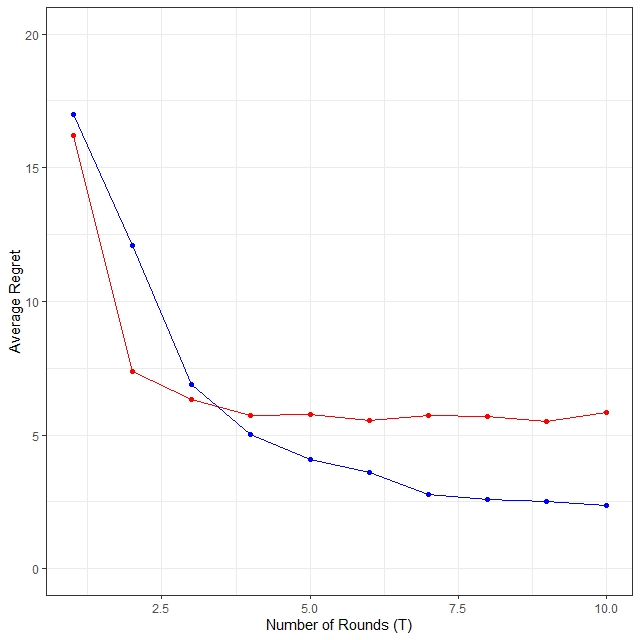
\includegraphics[width = \textwidth]{figT10.jpeg}
        \caption{$T = 10$}
    \end{subfigure}
    \begin{subfigure}{0.33\textwidth}
        \centering
        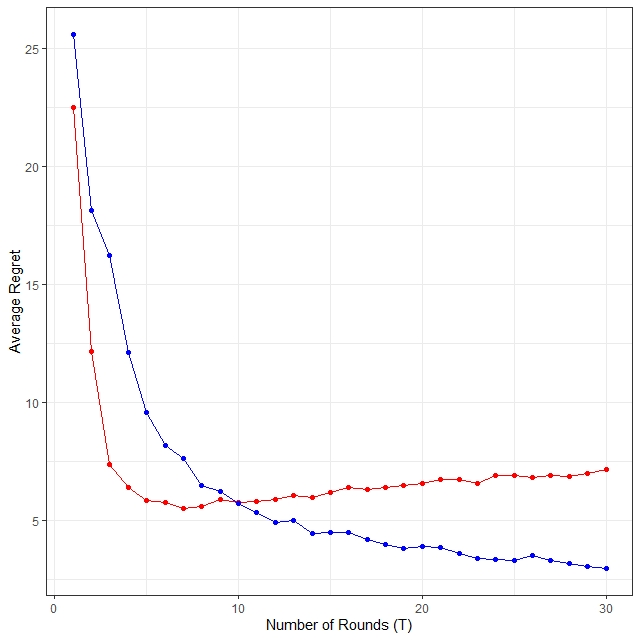
\includegraphics[width = \textwidth]{figT30.jpeg}
        \caption{$T = 30$}
    \end{subfigure}
    \begin{subfigure}{0.33\textwidth}
        \centering
        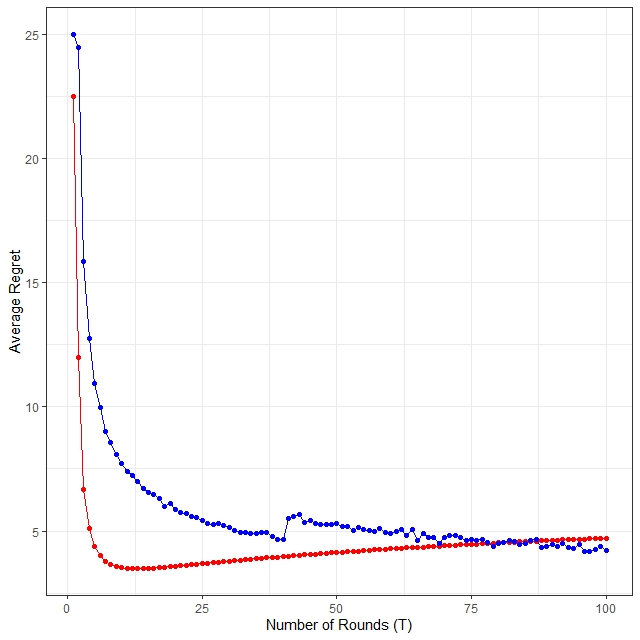
\includegraphics[width = \textwidth]{figT100.jpeg}
        \caption{$T = 100$}
    \end{subfigure}
    \caption{Average regret using ARC algorithm and our algorithm for dynamic pricing setup with dynamic latent variable. Red curve is the regret for ARC algorithm while blue curve is the regret for the new algorithm.}
    \label{fig:mainplot}
\end{figure}

From the simulation results, several conclusions may be drawn.

\begin{enumerate}
    \item For small values of $T$, our modified algorithm improves over ARC algorithm. 
    \item Since the underlying latent variable is not static (hence the assumption in ARC algorithm is violated), we see that it is not necessarily optimal. In the first few rounds, the latent parameter is changed only slightly, hence ARC algorithm performs greatly. But in the later round, it continues to choose the most rewarding price without concerning the inference regarding the change in public preferences. Therefore, the regrest increases.
    \item As $T$ increases, the objective mentioned in Eq.~\eqref{eqn:Rt-objective} becomes close to the objective concerned in ARC algorithm. Therefore, the exact round where our modification has an advantage over the ARC algorithm becomes large.
\end{enumerate}


\section{Conclusion}

The proposed modification of the Asymptotic Randomized Control algorithm is developed with the finite round optimality in mind. While the asymptotic nature of the posterior distributions is preserved through the usage of the central limit theorem, a finite round extension enables us to use a numerical technique like backward induction to solve the $k$-arm bandit problem. In turn, a more general version of the bandit problem is introduced, where the arms are correlated by a hyperparameter $X_t$, which is time-dependent, and evolves according to a rule governed by the action one takes at time $t$. In other words, this enables the slot machines (environment) to also strategize to some extent to counter the gambler's optimal strategy and its exploitation.

There are clearly a reasonable amount of memory constraints for this method, since, in the backward induction step, all the future possibilities must be calculated beforehand and used in the calculation of the optimal action at the current time. Also, due to the dynamic nature of the latent parameter $X_t$, the optimal actions are changed quite frequently to counter against changing $X_t$. However, in some practical scenario, consider a company choosing between several ad banners and showing the banner on a billboard, it may be costly to frequently change the banners. Therefore, one may need to restrict $\sum_{t=1}^{T-1} \ind{a_t \neq a_{t+1}}$ to some reasonable value. However, there is no immediate way to incorporate that in the modified algorithm.


\bibliographystyle{plain}
\bibliography{references.bib}

\end{document}